\documentclass[12pt]{article}

\usepackage{sbc-template}

\usepackage{graphicx,url}
\usepackage{amsmath}
\usepackage{float}
\usepackage[brazil]{babel}
%\usepackage[latin1]{inputenc}
\usepackage[utf8]{inputenc}
% UTF-8 encoding is recommended by ShareLaTex


\sloppy

\title{A study on the numerical methods to solve the n-body problem\\Symplectic Integrators}

\author{Gil S. M. Neto}


\address{Instituto de Matemática - Departamento de Matemática Aplicada\\ Universidade Federal do Rio de Janeiro
  (UFRJ)\\
 Rio de Janeiro -- RJ -- Brazil
  \email{gil.neto@ufrj.br}
}

\begin{document}

\maketitle

\begin{abstract}
  This is a study on the numerical solutions for the n-body problem, modeling
  the solar system and solving Newton's Law of Gravity for the position of the planets we can take a look on how different numerical approaches behaves on this system.\\

\end{abstract}

\section{Introduction}
One might be interested in how a determined particle moves along other particles, how to determine how this system of particles evolve? If we are talking about particles, or bodies, in the macroscopic world we should take a look at Newton's Law of Universal Gravitation\\
\[
F = G \frac{m_1m_2}{r^2}
\]
Where \(G = 6.67428 \cdot 10^{-11} \frac{m^3}{kg\cdot s^2}\) is the Gravitational constant, \(m_1\) is the mass of the first body, typically the body that we are interested in the position, \(m_2\) is the body interacting with our desired body, and \(r\) is the distance between the bodies.\\
But how can this equation be of any help to determine a body position? Well, combining this with Newton's Second Law of Motion
\[
F = ma
\]
We get
\begin{align*}
m_1a &= G \frac{m_1m_2}{r^2}\\
a &= G \frac{m_2}{r^2}
\end{align*}
But acceleration is just the second derivative of position, so what we truly have is the differential equation
\[
\ddot{r} = G \frac{m_2}{\lVert r \rVert^2}
\]
So, by transforming this into an initial value problem we can solve for the body's position.\\
The N-Body problem is a well know problem, the equations described above only tells us about a system of two bodies. But what about systems with more bodies? How to simulate a galaxy, for example, or how to determine where a GPS satellite must be in Earth's orbit?\\
This article is a case study of the N-Body problem, where N = 9, so we have the sun and the eight planets of the solar system (sorry Pluto). And we will take a look at how to model Newton's Equation of Motion on the computer, as a system of linear differential equations that we can solve.
\section{One Differential Equation to rule them all} \label{sec:thediffeq}
(...) One Differential Equation to find them all. And inspired by a Lord of The Rings line, we can use our One Differential Equation to determine all bodies' position.
\[
\ddot{r} = G \frac{m_2}{\lVert r \rVert^2}
\]
Rewriting this as a system of first order linear equations:
\begin{align*}
  \begin{cases}
    \dot{r} = v \\
    \ddot{v} = G \frac{m_2}{\lVert r \rVert^2}
  \end{cases}
\end{align*}
Give us an easy way to determine a body's position. But we are dealing with a system of 9 bodies, so the force acting on our main body is the sum of all forces from all the bodies, and our differential equation for the i-th body is:
\[
\ddot{r_i} = G\sum_{j=1}^{8}\left(\frac{m_j}{\lVert r_j \rVert^2}\right), j \neq i
\]
And our system of equations to solve becomes
\begin{align*}
  \begin{cases}
    \dot{r} = v \\
    \ddot{v} = G (\frac{m_1}{\lVert r_1 \rVert^2}\right + \frac{m_2}{\lVert r_2 \rVert^2}\right + \dots + \frac{m_8}{\lVert r_8 \rVert^2})
  \end{cases}
\end{align*}
Solving this for each planet gives us all the position of planets in the solar system.
\section{The Pyshics of the problem}
Going through the Physics Laws of the problem will give us tools to verify if our model is a good model, and if the numerical solutions are, in fact, solving the right model.

\subsection{Hamiltonian and Angular Momentum}
This system under Newton's Law is a conservative system, in other words, it conserves energy, as Professor Alan Sokal from University College London says, and we can look at the Hamiltonian of the system.\\
Here \(q\) denotes position vector, so \(\dot{q}\) is the velocity vector. \\
First of all, the self potential energy
\[
U = G \displaystyle \sum_{i,j}^n \frac{m_i m_j}{\lVert q_i - q_j \rVert}
\]
The linear momentum
\[
p_i = m_i \dot{q_i}
\]
And finally the Hamiltonian
\[
H = \displaystyle \sum_{i = 1}^{n} \frac{\lVert p_i \rVert ^2}{2m_i} - U
\]
And so \(H\) is constant.\\ yy 
Another conserved quantity is the Angular Momentum, which is defined as:
\[
L = r \times p
\]
\(r\) begin the position vector and \(p = mv\) the linear momentum vector.\\
We can simplify the equation for an easy one to solve
\begin{align*}
  L &= r \times p\\
  \lVert L \rVert &= \sqrt{\rVert r \lVert^2 \rVert p \lVert^2(sin(\theta))^2} \\
  &= \sqrt{\rVert r \lVert^2 \rVert p \lVert^2 - \rVert r \lVert^2 \rVert p \lVert^2(cos(\theta))^2} \\
  &= \sqrt{\rVert r \lVert^2 \rVert p \lVert^2 - \langle r, p \rangle ^2}
\end{align*}
In the second step we used the trigonometric identity \(sin^2 (t) + cos^2(t) = 1\), and in the third step \(\langle \cdot \rangle\) stands for the scalar product.\\
With this in mind, we expect that the numerical method for solving the n-body problem also conserves Energy and Angular Momentum.

\subsection{Kepler's Law}
\begin{enumerate}
  \item Planets move around the Sun in ellipses, with the Sun at one focus
  \item The line connecting the Sun to a planet sweeps equal areas in equal times
  \item The square of the orbital period of a planet is proportional to the cube of the mean distance from the Sun
\end{enumerate}
\subsubsection{First Law}
For the first Law, we will check for the eccentricity \(\epsilon \) of the orbits, if \(\lvert \epsilon \rvert < 1\) the orbit is indeed an ellipse. Also we will compare the numerical result of eccentricity to the data from NASA about the orbits.\\
Working on some Analytical Geometry, eccentricity is given by:
\[
\epsilon = \frac{ap - pe}{ap + pe}
\]
Where \(ap\) is the Aphelion (i.e. the furthest distance to the Sun) distance, \(pe\) is the Perihelion (i.e. the closest distance to the Sun) distance

\section{The numerical methods}
Given the energy conservative nature of the problem, the Euler Method and Runge-Kutta methods won't give us satisfactory results, because they don't conserve energies. Methods that conserves energy are called Symplectic methods.
In this article we will make use of the non-symplectics:
\begin{itemize}
  \item Euler (First Order)
\end{itemize}
 and the symplectic ones:
 \begin{itemize}
   \item Semi implicit Euler (Euler-Cromer - Second Order)
   \item 3 Step Verlet Integrator (Leapfrog - Second Order)
   \item 7 Step Verlet Integrator (Leapfrog - Higher Order)
 \end{itemize}
  \(V(t, x), A(t, x)\) are the velocity and acceleration at time \(t\) and position \(x(t)\), \(x_t\) is the position at time \(t\), \(v_t\) is the velocity at time \(t \), \(h\) is the time step.
 \subsubsection{Euler}
 \begin{align*}
   x_{t+1} &= x_t + h v_t\\
   v_{t+1} &= v_t + h a_t
 \end{align*}
 \subsubsection{Euler-Cromer}
 \begin{align*}
  v_{t+1} &= v_t + h a_t \\
  x_{t+1} &= x_t + h v_{t+1}
 \end{align*}
 \subsection{Velocity-Verlet}
 3 Step Verlet comes in two flavors, Velocity-Verlet and Position-Verlet, they yield the same results, so we will deal only with the velocity version, position one can be found in the source code.\\
 \begin{align*}
  v_{t+\frac{1}{2}} &= v_t + \frac{1}{2} h a_t \\
  x_{t+1} &= x_t + h v_{t+\frac{1}{2}}\\
  v_{t+1} &= v_{t+\frac{1}{2}} + \frac{1}{2} h A(t+1, x_{t+1})
 \end{align*}

 \subsection{7 Step Verlet - Leapfrog Integrator}
 \begin{align*}
  w &= \sqrt[3]{2}\\
  f &= 2 - w\\
  leap_1 = leap_7 &= \frac{h}{2f}\\
  leap_2 = leap_6 &= \frac{h}{f}\\
  leap_3 = leap_5 &= (1-w) \frac{h}{2f}\\
  leap_4 &= -h \frac{w}{f}\\
  x_{1} &= x_t + leap_1 \cdot v_t\\
  v_{2} &= v_t + leap__2 \cdot A(x_{1})\\
  x_{3} &= x_{1} + leap_3 \cdot v_{2}\\
  v_{4} &= v_{2} + leap_4 \cdot A(x{3})\\
  x_{5} &= x_{3} + leap_5 \cdot v_{4}\\
  v_{t+1} &= v_{4} + leap_6 \cdot A(x_{5})\\
  x_{t+1} &= x_{5} + leap_7 \cdot v_{t+1}
 \end{align*}

\section{Results}\label{sec:figs}
Now we will look at some results, the initial values for the simulation where choosen as: initial \(x\) coordinate: Aphelion distance; initial \(y\) coordinate: 0; initial velocity: Data from NASA Fact Sheet. The time step \(h\) is measured in seconds, \(h = 3600\) means \(1\) hour step.

\begin{figure}[H]
  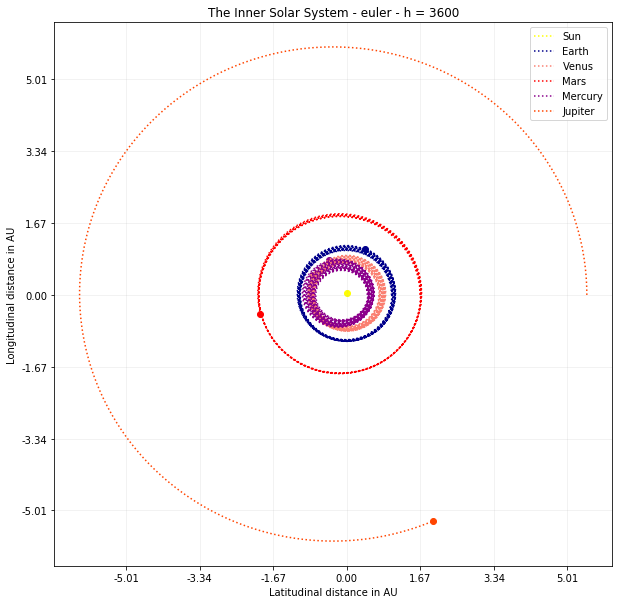
\includegraphics[width=.4\textwidth, height =.3\textheight]{euler-3600-orbit.png}
  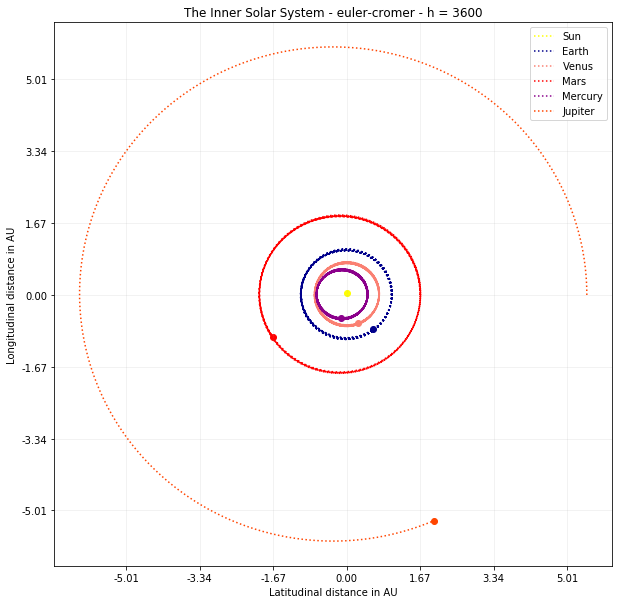
\includegraphics[width=.4\textwidth, height =.3\textheight]{eulercromer-3600-orbit.png}

  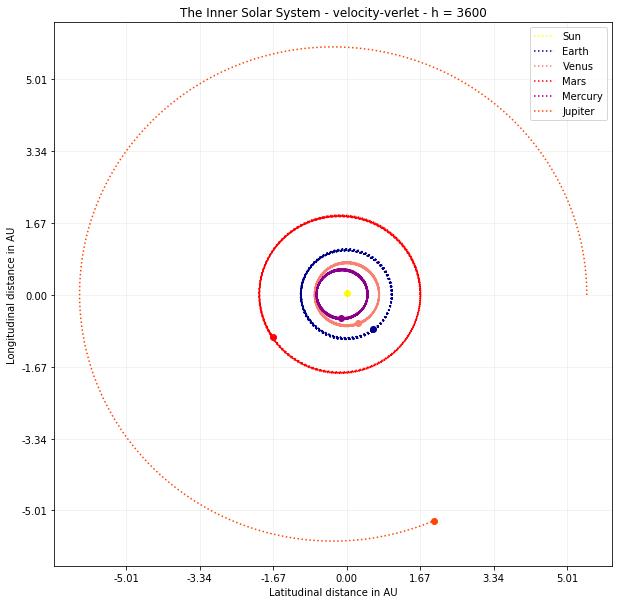
\includegraphics[width=.4\textwidth, height =.3\textheight]{verlet-3600-orbit.png}
  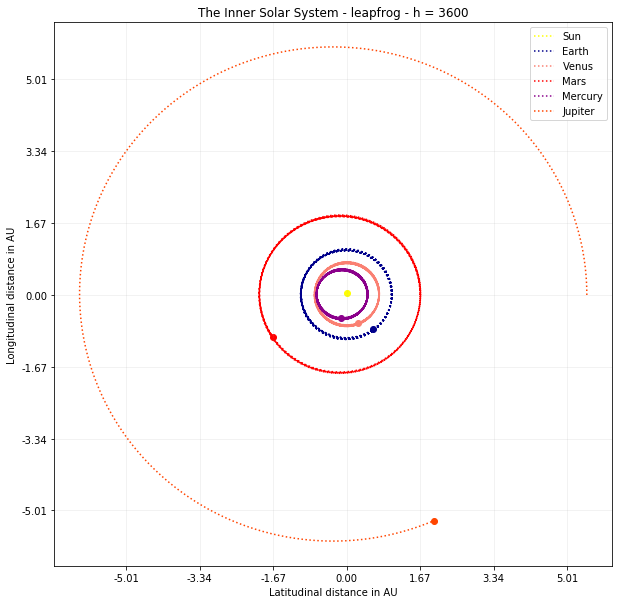
\includegraphics[width=.4\textwidth, height =.3\textheight]{leapfrog-3600-orbit.png}
  \caption{Orbits for \(h = 3600\) and simulated \(100000\) times (\(\approx 4100\) days)}
  \label{Euler Method}
\end{figure}
Just as the picture shows, the Euler Method gets off orbit, and the symplectic ones stay in orbit.
Now let's take a look at the Energy.
\begin{figure}[H]
  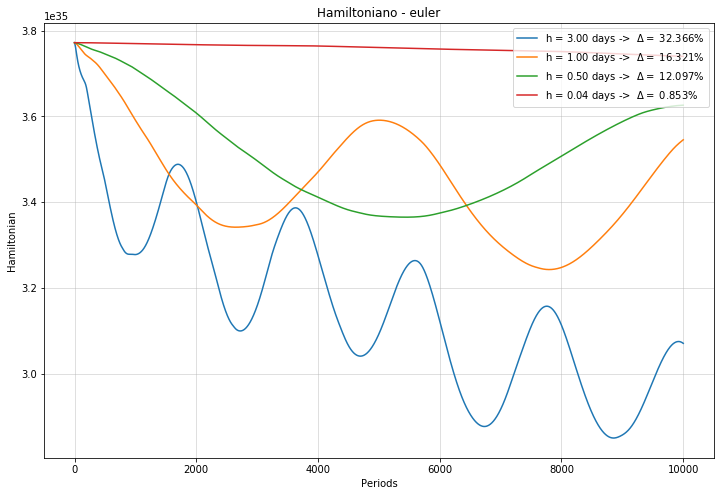
\includegraphics[width=.92\textwidth, height =.5\textheight]{h_euler.png}

  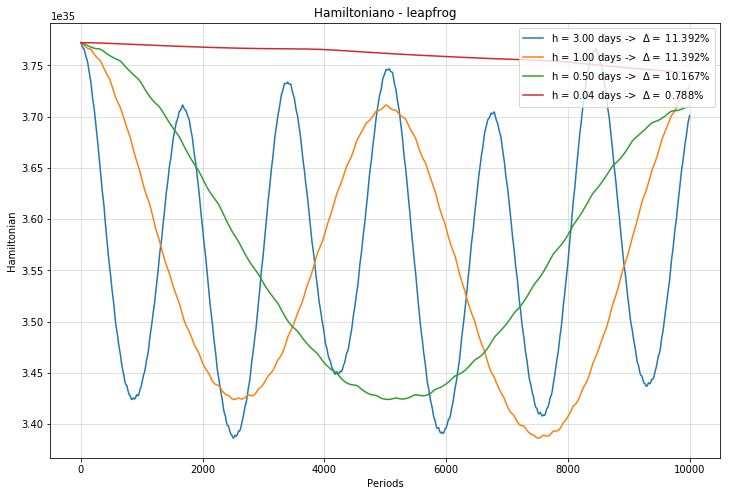
\includegraphics[width=.92\textwidth, height =.5\textheight]{h_leap.png}
  \caption{Mechanical Energy simulated \(100000\) times}
  \label{Euler Method}
\end{figure}
\begin{figure}[H]
  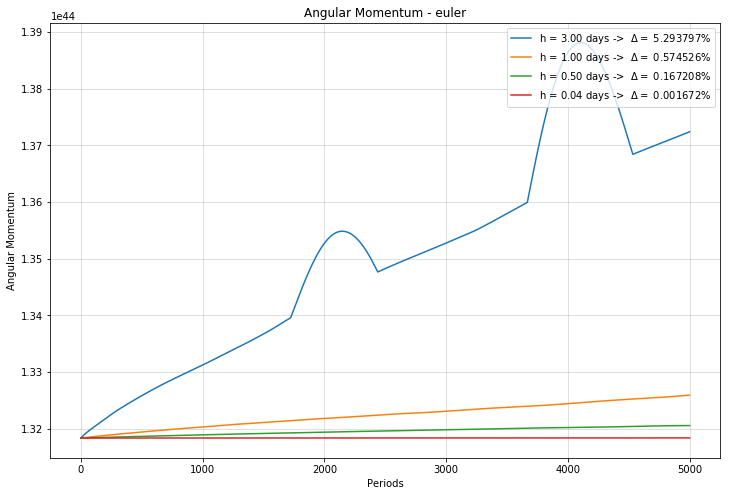
\includegraphics[width=.92\textwidth, height =.5\textheight]{an_euler.png}

  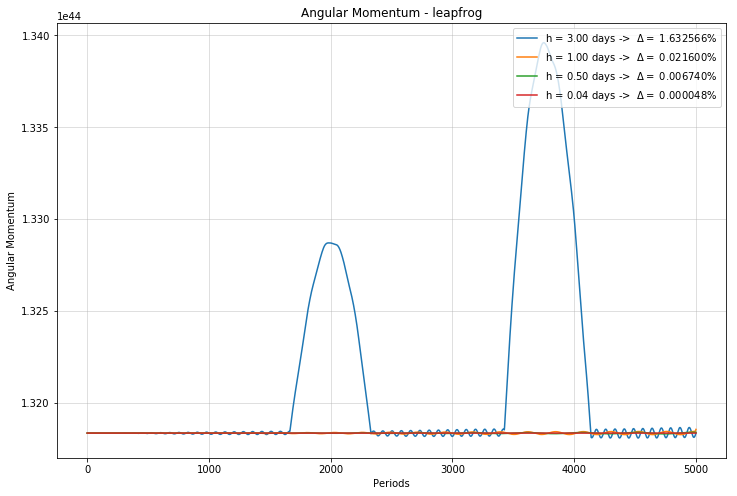
\includegraphics[width=.92\textwidth, height =.5\textheight]{an_leap.png}
  \caption{Angular momentum simulated \(40000\) times)}
  \label{Euler Method}
\end{figure}
The symplectic methods conserves the hamiltonian with bigger steps while euler methods only conserves with really small steps, also the hamiltonian with euler method is decreasing and not only a senoidal movement, while the leapfrog hamiltonian is bounded.\\
On the angular momentum graphs we can see this same characteristic.

\begin{table}[H]
\centering
\caption{Eccentricity values comparison for Kepler's third Law}
\label{tab:exTable1}
\smallskip
\begin{tabular}{|l|c|c|}
\hline
& Leapfrog Value & NASA Data\\[0.5ex]
\hline
&&\\[-2ex]
Mercury & 0.196 & 0.206\\[0.5ex]
\hline
&&\\[-2ex]
Venus & 0.018 & 0.007\\[0.5ex]
\hline
&&\\[-2ex]
Earth & 0.0164 & 0.017\\[0.5ex]
\hline
&&\\[-2ex]
Mars & 0.09 & 0.093\\[0.5ex]
\hline
&&\\[-2ex]
Jupiter & 0.05 & 0.048\\[0.5ex]
\hline
\end{tabular}
\end{table}
And so, our Model is pretty close from the pyshical data.
\section{Conclusion and links}
While the model and algorithm can be improved, like it's velocity (100000 simulations took 25 minutes on a i7 computer), we can really see the differences between the Symplectic and non-symplectic methods.\\
The 7 step Leapfrog has complexity \(\mathcal{O}(n^2)\), there's an algorithm worth mentioning: Barnes-Hut algorithm because it has complexity \(\mathcal{O}(\log{}n)\), it's widely used and it's main principle is to group distant bodies into one big body, so you reduce the amount of calculations.\\
Links for the souce code of the simulation can be found in \url{https://github.com/mirandagil/university-courses/tree/master/analise-numerica-edo-2019-1/project}

\begin{figure}[H]
  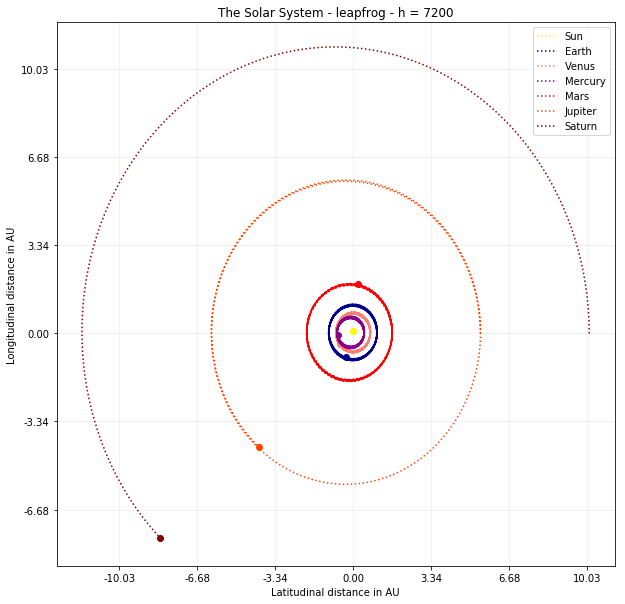
\includegraphics[width=.7\textwidth, height =.4\textheight]{planets.png}
  \caption{Leapfrog simulation with \( h = 7200 \) simulated \(100000\) times}
  \label{Euler Method}
\end{figure}

\section{References}
\begin{thebibliography}{9}
\bibitem{latexcompanion}
Alan Sokal.
\textit{Notes on MATH 0054 - Analytical Dynamics - University College London}.
\url{https://www.ucl.ac.uk/~ucahad0/}.

\bibitem{latexcompanion2}
Peter Young.
\textit{Notes on Computational Physics - University of California}.
\url{https://young.physics.ucsc.edu/115/}.

\bibitem{latexcompanion3}
Brian Tyrrell
\textit{Using numerical methods to solve the Gravitational n-Body Problem & represent the result graphically using OpenGL}.
\url{https://www.maths.tcd.ie/~btyrrel/nbody.pdf}.

\bibitem{knuthwebsite}
Planetary Fact Sheet - NASA,
\\\texttt{https://nssdc.gsfc.nasa.gov/planetary/factsheet/index.html}

\bibitem{knu2thwebsite}
MITx: 8.01.2x Mechanics: Momentum and Energy
\\\texttt{https://courses.edx.org/courses/course-v1:MITx+8.01.2x+3T2018/course/}
\end{thebibliography}


\end{document}
